% Options for packages loaded elsewhere
\PassOptionsToPackage{unicode}{hyperref}
\PassOptionsToPackage{hyphens}{url}
%
\documentclass[
]{article}
\usepackage{lmodern}
\usepackage{amssymb,amsmath}
\usepackage{ifxetex,ifluatex}
\ifnum 0\ifxetex 1\fi\ifluatex 1\fi=0 % if pdftex
  \usepackage[T1]{fontenc}
  \usepackage[utf8]{inputenc}
  \usepackage{textcomp} % provide euro and other symbols
\else % if luatex or xetex
  \usepackage{unicode-math}
  \defaultfontfeatures{Scale=MatchLowercase}
  \defaultfontfeatures[\rmfamily]{Ligatures=TeX,Scale=1}
\fi
% Use upquote if available, for straight quotes in verbatim environments
\IfFileExists{upquote.sty}{\usepackage{upquote}}{}
\IfFileExists{microtype.sty}{% use microtype if available
  \usepackage[]{microtype}
  \UseMicrotypeSet[protrusion]{basicmath} % disable protrusion for tt fonts
}{}
\makeatletter
\@ifundefined{KOMAClassName}{% if non-KOMA class
  \IfFileExists{parskip.sty}{%
    \usepackage{parskip}
  }{% else
    \setlength{\parindent}{0pt}
    \setlength{\parskip}{6pt plus 2pt minus 1pt}}
}{% if KOMA class
  \KOMAoptions{parskip=half}}
\makeatother
\usepackage{xcolor}
\IfFileExists{xurl.sty}{\usepackage{xurl}}{} % add URL line breaks if available
\IfFileExists{bookmark.sty}{\usepackage{bookmark}}{\usepackage{hyperref}}
\hypersetup{
  hidelinks,
  pdfcreator={LaTeX via pandoc}}
\urlstyle{same} % disable monospaced font for URLs
\usepackage[margin=1in]{geometry}
\usepackage{color}
\usepackage{fancyvrb}
\newcommand{\VerbBar}{|}
\newcommand{\VERB}{\Verb[commandchars=\\\{\}]}
\DefineVerbatimEnvironment{Highlighting}{Verbatim}{commandchars=\\\{\}}
% Add ',fontsize=\small' for more characters per line
\usepackage{framed}
\definecolor{shadecolor}{RGB}{248,248,248}
\newenvironment{Shaded}{\begin{snugshade}}{\end{snugshade}}
\newcommand{\AlertTok}[1]{\textcolor[rgb]{0.94,0.16,0.16}{#1}}
\newcommand{\AnnotationTok}[1]{\textcolor[rgb]{0.56,0.35,0.01}{\textbf{\textit{#1}}}}
\newcommand{\AttributeTok}[1]{\textcolor[rgb]{0.77,0.63,0.00}{#1}}
\newcommand{\BaseNTok}[1]{\textcolor[rgb]{0.00,0.00,0.81}{#1}}
\newcommand{\BuiltInTok}[1]{#1}
\newcommand{\CharTok}[1]{\textcolor[rgb]{0.31,0.60,0.02}{#1}}
\newcommand{\CommentTok}[1]{\textcolor[rgb]{0.56,0.35,0.01}{\textit{#1}}}
\newcommand{\CommentVarTok}[1]{\textcolor[rgb]{0.56,0.35,0.01}{\textbf{\textit{#1}}}}
\newcommand{\ConstantTok}[1]{\textcolor[rgb]{0.00,0.00,0.00}{#1}}
\newcommand{\ControlFlowTok}[1]{\textcolor[rgb]{0.13,0.29,0.53}{\textbf{#1}}}
\newcommand{\DataTypeTok}[1]{\textcolor[rgb]{0.13,0.29,0.53}{#1}}
\newcommand{\DecValTok}[1]{\textcolor[rgb]{0.00,0.00,0.81}{#1}}
\newcommand{\DocumentationTok}[1]{\textcolor[rgb]{0.56,0.35,0.01}{\textbf{\textit{#1}}}}
\newcommand{\ErrorTok}[1]{\textcolor[rgb]{0.64,0.00,0.00}{\textbf{#1}}}
\newcommand{\ExtensionTok}[1]{#1}
\newcommand{\FloatTok}[1]{\textcolor[rgb]{0.00,0.00,0.81}{#1}}
\newcommand{\FunctionTok}[1]{\textcolor[rgb]{0.00,0.00,0.00}{#1}}
\newcommand{\ImportTok}[1]{#1}
\newcommand{\InformationTok}[1]{\textcolor[rgb]{0.56,0.35,0.01}{\textbf{\textit{#1}}}}
\newcommand{\KeywordTok}[1]{\textcolor[rgb]{0.13,0.29,0.53}{\textbf{#1}}}
\newcommand{\NormalTok}[1]{#1}
\newcommand{\OperatorTok}[1]{\textcolor[rgb]{0.81,0.36,0.00}{\textbf{#1}}}
\newcommand{\OtherTok}[1]{\textcolor[rgb]{0.56,0.35,0.01}{#1}}
\newcommand{\PreprocessorTok}[1]{\textcolor[rgb]{0.56,0.35,0.01}{\textit{#1}}}
\newcommand{\RegionMarkerTok}[1]{#1}
\newcommand{\SpecialCharTok}[1]{\textcolor[rgb]{0.00,0.00,0.00}{#1}}
\newcommand{\SpecialStringTok}[1]{\textcolor[rgb]{0.31,0.60,0.02}{#1}}
\newcommand{\StringTok}[1]{\textcolor[rgb]{0.31,0.60,0.02}{#1}}
\newcommand{\VariableTok}[1]{\textcolor[rgb]{0.00,0.00,0.00}{#1}}
\newcommand{\VerbatimStringTok}[1]{\textcolor[rgb]{0.31,0.60,0.02}{#1}}
\newcommand{\WarningTok}[1]{\textcolor[rgb]{0.56,0.35,0.01}{\textbf{\textit{#1}}}}
\usepackage{longtable,booktabs}
% Correct order of tables after \paragraph or \subparagraph
\usepackage{etoolbox}
\makeatletter
\patchcmd\longtable{\par}{\if@noskipsec\mbox{}\fi\par}{}{}
\makeatother
% Allow footnotes in longtable head/foot
\IfFileExists{footnotehyper.sty}{\usepackage{footnotehyper}}{\usepackage{footnote}}
\makesavenoteenv{longtable}
\usepackage{graphicx,grffile}
\makeatletter
\def\maxwidth{\ifdim\Gin@nat@width>\linewidth\linewidth\else\Gin@nat@width\fi}
\def\maxheight{\ifdim\Gin@nat@height>\textheight\textheight\else\Gin@nat@height\fi}
\makeatother
% Scale images if necessary, so that they will not overflow the page
% margins by default, and it is still possible to overwrite the defaults
% using explicit options in \includegraphics[width, height, ...]{}
\setkeys{Gin}{width=\maxwidth,height=\maxheight,keepaspectratio}
% Set default figure placement to htbp
\makeatletter
\def\fps@figure{htbp}
\makeatother
\setlength{\emergencystretch}{3em} % prevent overfull lines
\providecommand{\tightlist}{%
  \setlength{\itemsep}{0pt}\setlength{\parskip}{0pt}}
\setcounter{secnumdepth}{-\maxdimen} % remove section numbering

\author{}
\date{\vspace{-2.5em}}

\begin{document}

\hypertarget{regression-analysis-for-motortrend}{%
\subsection{Regression Analysis For
MotorTrend}\label{regression-analysis-for-motortrend}}

The dataframe mtcars contains 32 observations on 11 variabels like
miles/gallon(MPG), number of cylinders etc.

Our main focus in the study is how the Transmission type( automatic or
manual) affects the miles per gallon. define a relationship between
mileage and transmission type.

\hypertarget{loading-and-the-data}{%
\subsubsection{Loading and the Data}\label{loading-and-the-data}}

\begin{Shaded}
\begin{Highlighting}[]
\KeywordTok{data}\NormalTok{(}\StringTok{"mtcars"}\NormalTok{)}
\NormalTok{mtcars <-}\StringTok{ }\NormalTok{mtcars}\OperatorTok
\StringTok{  }\KeywordTok{mutate}\NormalTok{(}\DataTypeTok{am =} \KeywordTok{as.factor}\NormalTok{ (am))}
\KeywordTok{levels}\NormalTok{(mtcars}\OperatorTok{$}\NormalTok{am)<-}\StringTok{ }\KeywordTok{c}\NormalTok{(}\StringTok{"Automatic"}\NormalTok{,}\StringTok{"Manual"}\NormalTok{)}

\KeywordTok{summary}\NormalTok{(mtcars)}
\end{Highlighting}
\end{Shaded}

\begin{verbatim}
##       mpg             cyl             disp             hp       
##  Min.   :10.40   Min.   :4.000   Min.   : 71.1   Min.   : 52.0  
##  1st Qu.:15.43   1st Qu.:4.000   1st Qu.:120.8   1st Qu.: 96.5  
##  Median :19.20   Median :6.000   Median :196.3   Median :123.0  
##  Mean   :20.09   Mean   :6.188   Mean   :230.7   Mean   :146.7  
##  3rd Qu.:22.80   3rd Qu.:8.000   3rd Qu.:326.0   3rd Qu.:180.0  
##  Max.   :33.90   Max.   :8.000   Max.   :472.0   Max.   :335.0  
##       drat             wt             qsec             vs        
##  Min.   :2.760   Min.   :1.513   Min.   :14.50   Min.   :0.0000  
##  1st Qu.:3.080   1st Qu.:2.581   1st Qu.:16.89   1st Qu.:0.0000  
##  Median :3.695   Median :3.325   Median :17.71   Median :0.0000  
##  Mean   :3.597   Mean   :3.217   Mean   :17.85   Mean   :0.4375  
##  3rd Qu.:3.920   3rd Qu.:3.610   3rd Qu.:18.90   3rd Qu.:1.0000  
##  Max.   :4.930   Max.   :5.424   Max.   :22.90   Max.   :1.0000  
##          am          gear            carb      
##  Automatic:19   Min.   :3.000   Min.   :1.000  
##  Manual   :13   1st Qu.:3.000   1st Qu.:2.000  
##                 Median :4.000   Median :2.000  
##                 Mean   :3.688   Mean   :2.812  
##                 3rd Qu.:4.000   3rd Qu.:4.000  
##                 Max.   :5.000   Max.   :8.000
\end{verbatim}

\hypertarget{exploratory-data-anlaysis}{%
\subsubsection{Exploratory Data
Anlaysis}\label{exploratory-data-anlaysis}}

The Displacement ,Mileage, HorsePower, axle ratio, quator mile time,
weight are all the continous variables.

And other varibles are categorical

And our only intrest is to find relationship between Transmission type
and Mileage.

we will analyse the continous variables sactter plot with mileage

\begin{Shaded}
\begin{Highlighting}[]
\NormalTok{ mtcars.con <-}\StringTok{ }\NormalTok{mtcars[}\KeywordTok{c}\NormalTok{(}\StringTok{"mpg"}\NormalTok{,}\StringTok{"disp"}\NormalTok{,}\StringTok{"hp"}\NormalTok{,}\StringTok{"drat"}\NormalTok{,}\StringTok{"wt"}\NormalTok{,   }\StringTok{"qsec"}\NormalTok{)]}
\NormalTok{my_cols <-}\StringTok{ }\KeywordTok{c}\NormalTok{(}\StringTok{"#00AFBB"}\NormalTok{, }\StringTok{"#E7B800"}\NormalTok{, }\StringTok{"#FC4E07"}\NormalTok{)  }
\KeywordTok{pairs}\NormalTok{(mtcars.con ,}\DataTypeTok{pch =} \DecValTok{19}\NormalTok{, }\DataTypeTok{cex =}\FloatTok{0.5}\NormalTok{, }\DataTypeTok{col =}\NormalTok{ my_cols[mtcars}\OperatorTok{$}\NormalTok{am], }\DataTypeTok{lower.panel =} \OtherTok{NULL}\NormalTok{, }\DataTypeTok{font.labels =} \DecValTok{2}\NormalTok{, }\DataTypeTok{cex.labels =} \FloatTok{1.3}\NormalTok{)}
\end{Highlighting}
\end{Shaded}

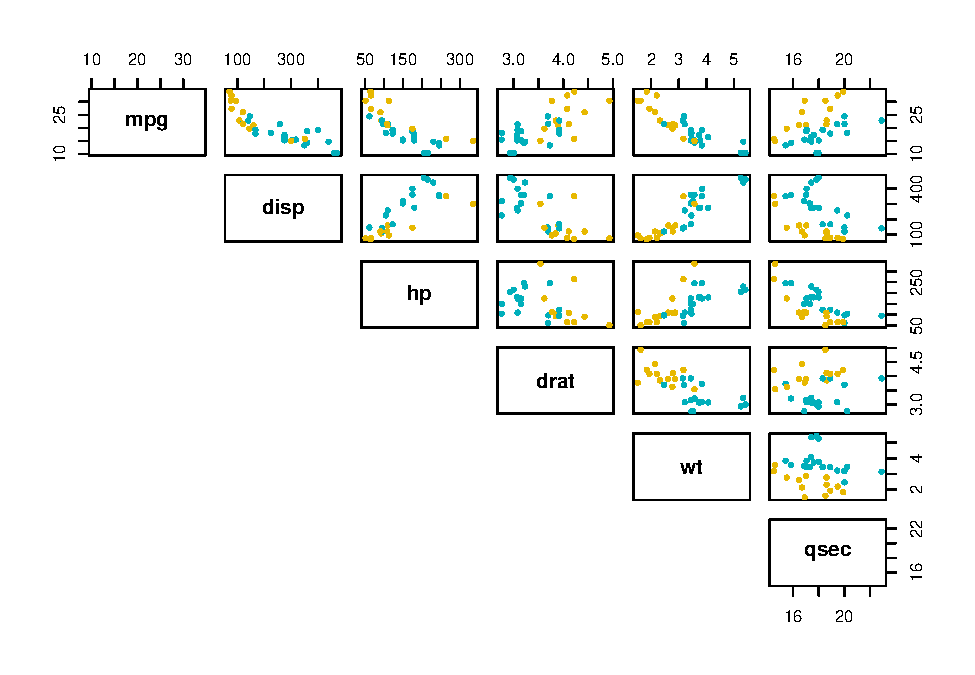
\includegraphics{MotorTrendAnalysis_files/figure-latex/pairPlots-1.pdf}

\begin{Shaded}
\begin{Highlighting}[]
\NormalTok{g <-}\StringTok{ }\KeywordTok{ggplot}\NormalTok{(}\DataTypeTok{data =}\NormalTok{ mtcars, }\KeywordTok{aes}\NormalTok{(}\DataTypeTok{x =}\NormalTok{ disp, }\DataTypeTok{y =}\NormalTok{ mpg, }\DataTypeTok{color =}\NormalTok{ am))}
\NormalTok{g <-}\StringTok{ }\NormalTok{g }\OperatorTok{+}\StringTok{ }\KeywordTok{geom_point}\NormalTok{( }\DataTypeTok{alpha =} \FloatTok{0.5}\NormalTok{)}
\NormalTok{g <-}\StringTok{ }\NormalTok{g }\OperatorTok{+}\StringTok{ }\KeywordTok{labs}\NormalTok{(}\DataTypeTok{x =} \StringTok{"Displacement in cubic inches"}\NormalTok{, }\DataTypeTok{y =} \StringTok{"Miles/(US) gallon"}\NormalTok{, }\DataTypeTok{title =} \StringTok{"Milege Vs Displacement"}\NormalTok{, }\DataTypeTok{color =} \StringTok{"Transmission Type"}\NormalTok{)}

\NormalTok{g1 <-}\StringTok{ }\KeywordTok{ggplot}\NormalTok{(}\DataTypeTok{data =}\NormalTok{ mtcars, }\KeywordTok{aes}\NormalTok{(}\DataTypeTok{x =}\NormalTok{ hp, }\DataTypeTok{y =}\NormalTok{ mpg, }\DataTypeTok{color =}\NormalTok{ am))}
\NormalTok{g1 <-}\StringTok{ }\NormalTok{g1 }\OperatorTok{+}\StringTok{ }\KeywordTok{geom_point}\NormalTok{( }\DataTypeTok{alpha =} \FloatTok{0.5}\NormalTok{)}
\NormalTok{g1 <-}\StringTok{ }\NormalTok{g1 }\OperatorTok{+}\StringTok{ }\KeywordTok{labs}\NormalTok{(}\DataTypeTok{x =} \StringTok{"Gross horse Power"}\NormalTok{, }\DataTypeTok{y =} \StringTok{"Miles/(US) gallon"}\NormalTok{, }\DataTypeTok{title =} \StringTok{"Milege Vs Gross HorsePower"}\NormalTok{, }\DataTypeTok{color =} \StringTok{"Type"}\NormalTok{)}

\NormalTok{g2 <-}\StringTok{ }\KeywordTok{ggplot}\NormalTok{(}\DataTypeTok{data =}\NormalTok{ mtcars, }\KeywordTok{aes}\NormalTok{(}\DataTypeTok{x =}\NormalTok{ wt, }\DataTypeTok{y =}\NormalTok{ mpg, }\DataTypeTok{color =}\NormalTok{ am))}
\NormalTok{g2 <-}\StringTok{ }\NormalTok{g2 }\OperatorTok{+}\StringTok{ }\KeywordTok{geom_point}\NormalTok{( }\DataTypeTok{alpha =} \FloatTok{0.5}\NormalTok{)}
\NormalTok{g2 <-}\StringTok{ }\NormalTok{g2 }\OperatorTok{+}\StringTok{ }\KeywordTok{labs}\NormalTok{(}\DataTypeTok{x =} \StringTok{"Weight in 1000 lbs"}\NormalTok{, }\DataTypeTok{y =} \StringTok{"Miles/(US) gallon"}\NormalTok{, }\DataTypeTok{title =} \StringTok{"Milege Vs Weight"}\NormalTok{,}\DataTypeTok{color =} \StringTok{"Type"}\NormalTok{)}

\NormalTok{g3 <-}\StringTok{ }\KeywordTok{ggplot}\NormalTok{(}\DataTypeTok{data =}\NormalTok{ mtcars, }\KeywordTok{aes}\NormalTok{(}\DataTypeTok{x =}\NormalTok{ drat, }\DataTypeTok{y =}\NormalTok{ mpg ,}\DataTypeTok{color =}\NormalTok{ am))}
\NormalTok{g3 <-}\StringTok{ }\NormalTok{g3 }\OperatorTok{+}\StringTok{ }\KeywordTok{geom_point}\NormalTok{( }\DataTypeTok{alpha =} \FloatTok{0.5}\NormalTok{ )}
\NormalTok{g3 <-}\StringTok{ }\NormalTok{g3 }\OperatorTok{+}\StringTok{ }\KeywordTok{labs}\NormalTok{(}\DataTypeTok{x =} \StringTok{"Rear axle ratio"}\NormalTok{, }\DataTypeTok{y =} \StringTok{"Miles/(US) gallon"}\NormalTok{, }\DataTypeTok{title =} \StringTok{"Milege Vs Rear axle ratio"}\NormalTok{, }\DataTypeTok{color =} \StringTok{"Type"}\NormalTok{)}


\NormalTok{g4 <-}\StringTok{ }\KeywordTok{ggplot}\NormalTok{(}\DataTypeTok{data =}\NormalTok{ mtcars, }\KeywordTok{aes}\NormalTok{(}\DataTypeTok{x =}\NormalTok{ qsec, }\DataTypeTok{y =}\NormalTok{ mpg ,}\DataTypeTok{color =}\NormalTok{ am))}
\NormalTok{g4 <-}\StringTok{ }\NormalTok{g4 }\OperatorTok{+}\StringTok{ }\KeywordTok{geom_point}\NormalTok{( }\DataTypeTok{alpha =} \FloatTok{0.5}\NormalTok{ )}
\NormalTok{g4 <-}\StringTok{ }\NormalTok{g4 }\OperatorTok{+}\StringTok{ }\KeywordTok{labs}\NormalTok{(}\DataTypeTok{x =} \StringTok{"Quator Mile Time"}\NormalTok{, }\DataTypeTok{y =} \StringTok{"Miles/(US) gallon"}\NormalTok{, }\DataTypeTok{title =} \StringTok{"Milege Vs Quator Mile Time"}\NormalTok{, }\DataTypeTok{color =} \StringTok{"Type"}\NormalTok{)}

\KeywordTok{ggarrange}\NormalTok{(g,g1,g2, g3,g4, }\DataTypeTok{ncol =} \DecValTok{2}\NormalTok{, }\DataTypeTok{nrow =} \DecValTok{3}\NormalTok{, }
          \DataTypeTok{common.legend =} \OtherTok{TRUE}\NormalTok{, }\DataTypeTok{legend =} \StringTok{"bottom"}\NormalTok{)}
\end{Highlighting}
\end{Shaded}

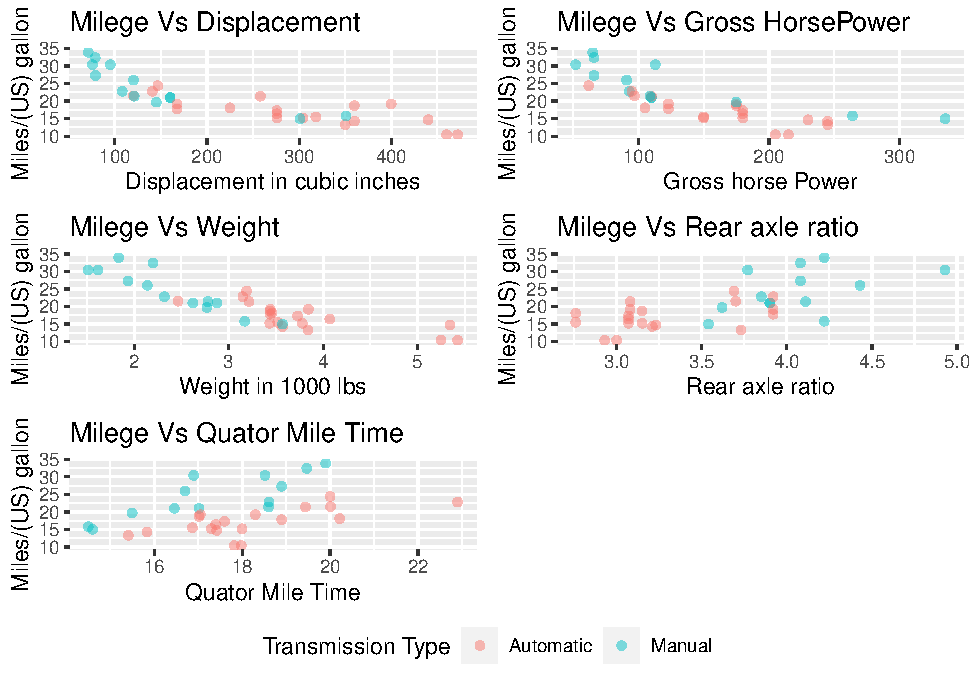
\includegraphics{MotorTrendAnalysis_files/figure-latex/exploartory analysis-1.pdf}

\begin{Shaded}
\begin{Highlighting}[]
\NormalTok{corr_disp<-}\StringTok{ }\KeywordTok{cor}\NormalTok{(mtcars}\OperatorTok{$}\NormalTok{disp , mtcars}\OperatorTok{$}\NormalTok{mpg)}
\NormalTok{corr_hp<-}\StringTok{ }\KeywordTok{cor}\NormalTok{(mtcars}\OperatorTok{$}\NormalTok{hp , mtcars}\OperatorTok{$}\NormalTok{mpg)}
\NormalTok{corr_wt<-}\StringTok{ }\KeywordTok{cor}\NormalTok{(mtcars}\OperatorTok{$}\NormalTok{wt , mtcars}\OperatorTok{$}\NormalTok{mpg)}
\NormalTok{corr_drat <-}\KeywordTok{cor}\NormalTok{(mtcars}\OperatorTok{$}\NormalTok{drat , mtcars}\OperatorTok{$}\NormalTok{mpg)}
\NormalTok{corr_qsec<-}\StringTok{ }\KeywordTok{cor}\NormalTok{(mtcars}\OperatorTok{$}\NormalTok{qsec , mtcars}\OperatorTok{$}\NormalTok{mpg)}
\end{Highlighting}
\end{Shaded}

** The Correlation values of the different relationship **

\begin{itemize}
\item
  The Plot shows a negative Trend with correlation values of
  \textbf{-0.848} between Displacement and Mileage.
\item
  The Plot shows a negative Trend with correlation values of
  \textbf{-0.776} between HosrePower and Mileage.
\item
  The Plot shows a negative Trend with correlation values of
  \textbf{-0.868} between weight and Mileage.
\item
  The Plot shows a postive Trend with correlation values of
  \textbf{0.681} between rear axle ratio and Mileage.
\item
  The Plot shows a postive Trend with correlation values of
  \textbf{0.419} between quator mile time and Mileage.
\end{itemize}

The Dependency of MPG value on Transmission Type is explained by the Bar
and Violin Plots.

\begin{Shaded}
\begin{Highlighting}[]
\NormalTok{l<-}\StringTok{ }\KeywordTok{labs}\NormalTok{(}\DataTypeTok{x =} \StringTok{"Transmission Type"}\NormalTok{, }\DataTypeTok{y =} \StringTok{"Mile Per Gallon"}\NormalTok{, }\DataTypeTok{fill =} \StringTok{"Transmission Type"}\NormalTok{)}
\NormalTok{box <-}\StringTok{ }\KeywordTok{ggplot}\NormalTok{(}\DataTypeTok{data =}\NormalTok{ mtcars, }\KeywordTok{aes}\NormalTok{(am , mpg, }\DataTypeTok{fill =}\NormalTok{ am))}
\NormalTok{box_plot <-}\StringTok{ }\NormalTok{box}\OperatorTok{+}\KeywordTok{geom_boxplot}\NormalTok{()}\OperatorTok{+}\NormalTok{l}
\NormalTok{violin <-}\StringTok{ }\NormalTok{box}\OperatorTok{+}\KeywordTok{geom_violin}\NormalTok{(}\DataTypeTok{color =} \StringTok{"black"}\NormalTok{, }\DataTypeTok{size =} \DecValTok{1}\NormalTok{)}\OperatorTok{+}\NormalTok{l}

\KeywordTok{ggarrange}\NormalTok{(box_plot, violin, }\DataTypeTok{ncol =} \DecValTok{2}\NormalTok{, }\DataTypeTok{common.legend =} \OtherTok{TRUE}\NormalTok{, }\DataTypeTok{legend =} \StringTok{"bottom"}\NormalTok{)}
\end{Highlighting}
\end{Shaded}

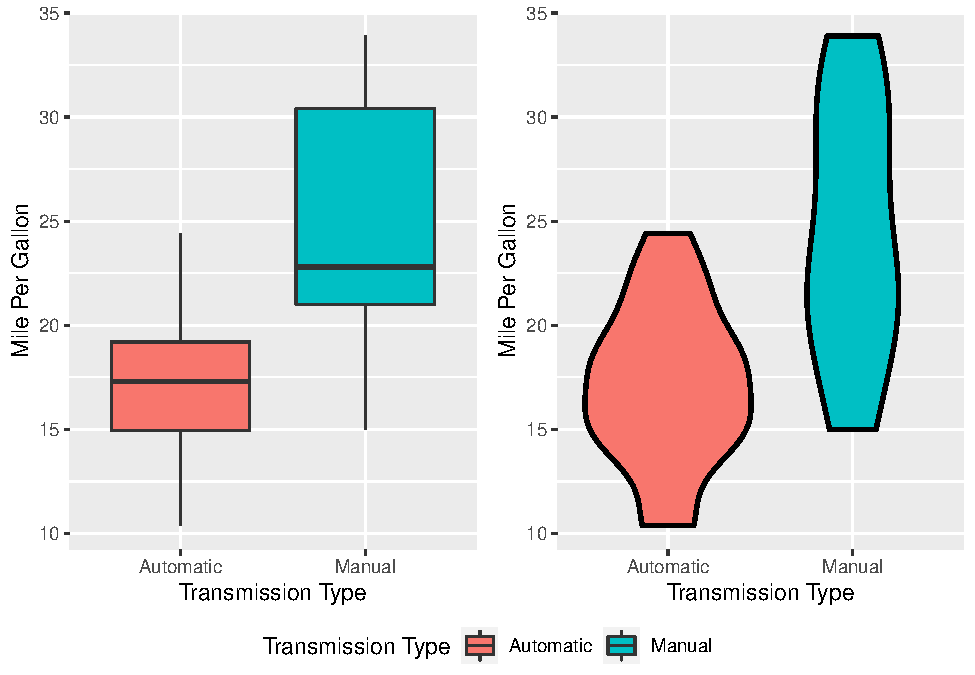
\includegraphics{MotorTrendAnalysis_files/figure-latex/unnamed-chunk-1-1.pdf}

The Box plot reveals that there is a huge differnce in mean mpg for the
automatic and manual Transmission

\begin{quote}
Since, Our question of analysis is relationship between the Mileage with
respect to transmission. And Displacement and Weight Shows high
correlation with Mileage.
\end{quote}

\begin{quote}
The Regression analysis of Mileage as outcome and Weight,Mileage and
Type as Predictors.
\end{quote}

\hypertarget{model-of-regression}{%
\subsubsection{Model of Regression}\label{model-of-regression}}

First to test the Transmission Type is really a categorical value to
determine the MPG.

\begin{Shaded}
\begin{Highlighting}[]
\KeywordTok{t.test}\NormalTok{(mtcars}\OperatorTok{$}\NormalTok{mpg}\OperatorTok{~}\NormalTok{mtcars}\OperatorTok{$}\NormalTok{am,}\DataTypeTok{conf.level=}\FloatTok{0.95}\NormalTok{)}
\end{Highlighting}
\end{Shaded}

\begin{verbatim}
## 
##  Welch Two Sample t-test
## 
## data:  mtcars$mpg by mtcars$am
## t = -3.7671, df = 18.332, p-value = 0.001374
## alternative hypothesis: true difference in means is not equal to 0
## 95 percent confidence interval:
##  -11.280194  -3.209684
## sample estimates:
## mean in group Automatic    mean in group Manual 
##                17.14737                24.39231
\end{verbatim}

The T-test rejects the null Hypothesis, the difference between
Transmission on MPG is 0.

\begin{Shaded}
\begin{Highlighting}[]
\NormalTok{mdl <-}\StringTok{ }\KeywordTok{lm}\NormalTok{(mpg}\OperatorTok{~}\NormalTok{disp}\OperatorTok{+}\NormalTok{wt}\OperatorTok{+}\NormalTok{am , }\DataTypeTok{data =}\NormalTok{ mtcars)}
\NormalTok{coef_mdl <-}\StringTok{ }\KeywordTok{coef}\NormalTok{(mdl)}
\NormalTok{rsquare_val <-}\StringTok{ }\KeywordTok{summary}\NormalTok{(mdl)}\OperatorTok{$}\NormalTok{adj.r.squared}
\end{Highlighting}
\end{Shaded}

\begin{itemize}
\tightlist
\item
  The adjusted R square value is \textbf{0.757583}
\end{itemize}

\begin{longtable}[]{@{}ll@{}}
\toprule
Feature & coeffcient value\tabularnewline
\midrule
\endhead
Intercept & 34.6759109\tabularnewline
displacement & -0.0178049\tabularnewline
Weight & -3.2790439\tabularnewline
manual transmission & 0.1777241\tabularnewline
\bottomrule
\end{longtable}

\hypertarget{model-selection}{%
\subsubsection{Model Selection}\label{model-selection}}

We can step method to as R to choose the best model itself

\begin{Shaded}
\begin{Highlighting}[]
\NormalTok{bestmodel =}\StringTok{ }\KeywordTok{step}\NormalTok{(}\KeywordTok{lm}\NormalTok{(mpg}\OperatorTok{~}\NormalTok{. , }\DataTypeTok{data =}\NormalTok{ mtcars), }\DataTypeTok{trace =} \DecValTok{0}\NormalTok{)}
\NormalTok{coef_bdl <-}\StringTok{ }\KeywordTok{coef}\NormalTok{(bestmodel)}
\NormalTok{rsquare_bval <-}\StringTok{ }\KeywordTok{summary}\NormalTok{(bestmodel)}\OperatorTok{$}\NormalTok{adj.r.squared}
\NormalTok{vif_model <-}\StringTok{ }\KeywordTok{vif}\NormalTok{(bestmodel)}
\end{Highlighting}
\end{Shaded}

\begin{itemize}
\item
  The BestModel that fits perfectly for MPG as outcome is with
  predictors Weight,Quator Mile time and Transmission Type.
\item
  The adjusted R square value for best model is \textbf{0.8335561}
\end{itemize}

\begin{longtable}[]{@{}lll@{}}
\toprule
Feature & coeffcient value & VIF\tabularnewline
\midrule
\endhead
Weight & -3.9165037 & 2.4829515\tabularnewline
Quator mile Time & 1.225886 & 1.3643391\tabularnewline
manual transmission & 2.9358372 & 2.5414372\tabularnewline
\bottomrule
\end{longtable}

The Residual Plots for the Fitted values and inputs

\begin{Shaded}
\begin{Highlighting}[]
\KeywordTok{par}\NormalTok{(}\DataTypeTok{mfrow =} \KeywordTok{c}\NormalTok{(}\DecValTok{2}\NormalTok{,}\DecValTok{2}\NormalTok{))}
\KeywordTok{plot}\NormalTok{(bestmodel)}
\end{Highlighting}
\end{Shaded}

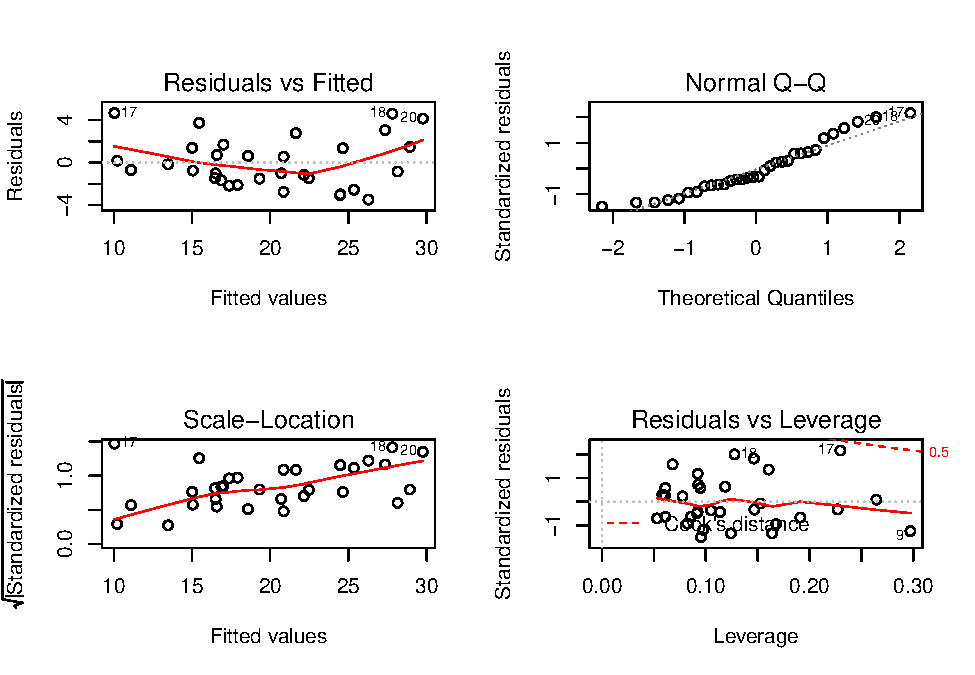
\includegraphics{MotorTrendAnalysis_files/figure-latex/unnamed-chunk-3-1.pdf}

\hypertarget{conclusion}{%
\subsubsection{Conclusion}\label{conclusion}}

Based on the previous analysis, we can say that on average manual
transmission is better than automatic transmission by 2.9 mpg but also
transmission type is not the only factor accounting for MPG, weight, and
acceleration (1/4 mile time) also needs to be considered.

\end{document}
